\section{Análisis a frecuencias medias}
\subsection{Cálculo teórico}

Para dichas frecuencias, se consideran los capacitores externos como cables (poseen una impedancia tan chica que se puede despreciar su efecto en estas frecuencias), mientras que las parásitas del integrado se consideran como abiertos. El esquema para este análisis puede verse en la figura \ref{im:frecuenciasMedias}.

\begin{figure}[ht]
	\centering
	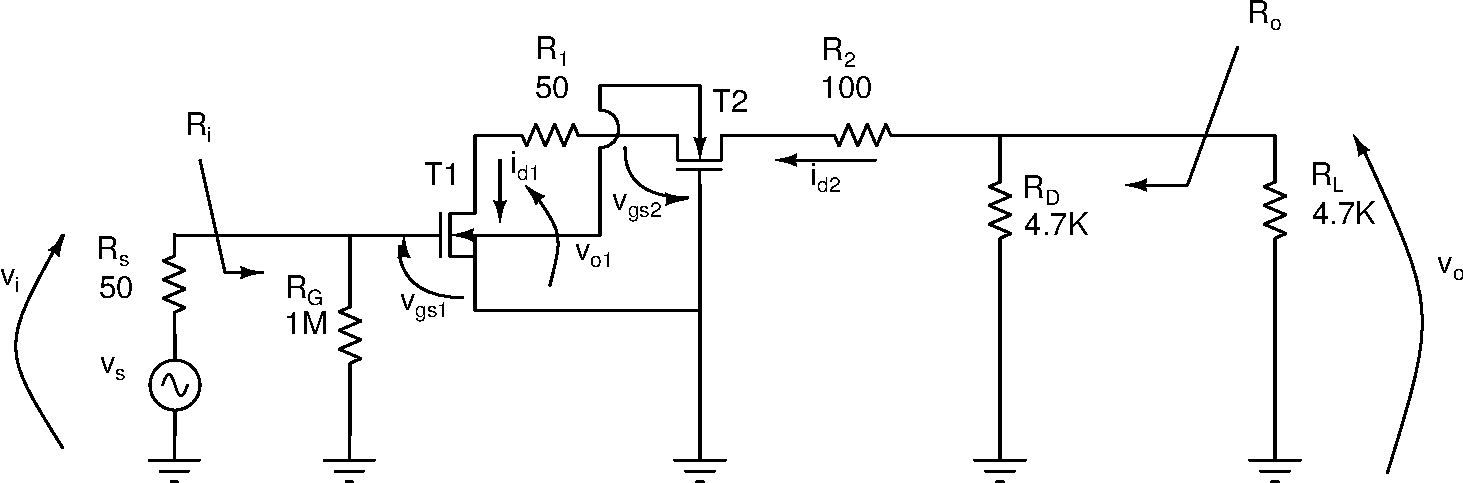
\includegraphics[scale=0.5]{../img/frecuenciasMedias.pdf}
	\caption{circuito amplificador a frecuencias medias.}
	\label{im:frecuenciasMedias}
\end{figure}

Con estos sentidos de referencias se procederá a calcular los parámetros de amplificación, además de obtener los valores de resistencias de entrada y salida.

La expresión de la ganancia de la etapa emisor común puede verse en la siguiente ecuación:

\begin{equation}
	A_{v1} = \frac{v_{o1}}{v_i} = \frac{-\id \cdot (50 +\Ridos)}{\vgs}
\end{equation}

La resistencia de entrada del transitor dos, $\Ridos$ vale:
\begin{equation}
	\Ridos = \frac{\rpi}{\hFET} = \frac{1}{\gmdos}
	\label{eq:Ri2}
\end{equation}

La ganancia del primer transistor entonces es de:

\begin{equation}
	A_{v1} =-\gmuno(\frac{1}{\gmdos}+50\ohm) = -0.5
	\label{eq:Av1}
\end{equation}

Esta ganancia, si bien es muy baja considerando que es un transistor en emisor común, resulta lógico, ya que como carga se está conectando un transitor base común, cuya característica principal es una resistencia de entrada muy baja. Para el transistor 2, se procede de la misma forma que con el transistor 1:

\begin{equation}
	A_{v2} = \frac{v_o}{v_{o1}} = \frac{- \id \cdot \mbox{R}_{ca}}{- \vgs - \id 50\ohm} = \frac{1}{\frac{1}{\gmdos}+50\ohm} \cdot 2.35\Kohm = 21.46
	\label{eq:Av2}
\end{equation}

La ganancia total del circuito es de $-10.73$.

Por inspección, los valores de la resistencias de entrada y de salida de todo el bloque son los siguientes:

\begin{equation}
	\Ri = 1\Mohm // \rgs = 1\Mohm 
\end{equation}

\begin{equation}
	\Ro = 4.5\Kohm // R_{oc} = 4.7\Kohm
\end{equation}

\begin{equation}
	R_{oc} = \ro \cdot (1 + \frac{\hFET \cdot R_s}{\rgs}) \rightarrow \infty
\end{equation}

Estos valores son los ideales. Cuando se simule, y sobre todo cuando se realicen las mediciones, los valores de las resistencias tenderán a cambiar, sobre todo la de entrada. Esto se debe a la influencia que tendrá el equivalente de la punta de osciloscopio.

Con estos valores calculados, se procederá a medir las máximas excursiones sin recorte. Para comenzar con esto, se admite que la entrada $\hat{\V}_{imax}$ es tal que no distorsiona por alinealidad. Para lograr esto, la señal de entrada debe cumplir:

\begin{equation}
	\hat{\V}_{ime sin distorosion} < \frac{\VGSQ - \VT}{2}
	\label{eq:viSinDistorsion}
\end{equation}

Para llegar a esta ecuación se debe partir de que la ecuación de la corriente de drain, aproximarla a una recta y buscar la ordenada al origen de esta recta, como se puede ver en la figura \ref{im:maximaExcursionSinDistorsion}.

\begin{figure}
	\centering
	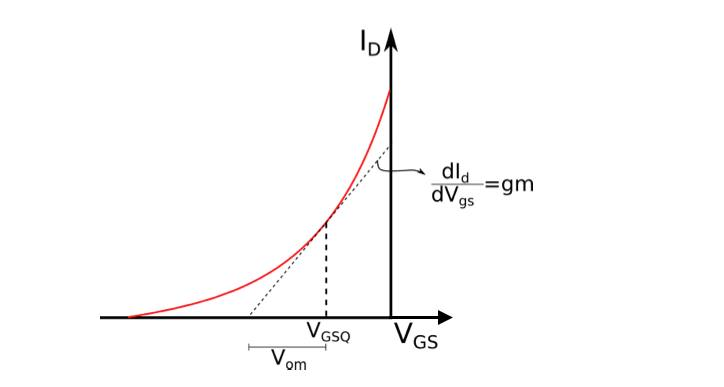
\includegraphics[scale=0.5]{../img/distorsion.jpg}
	\caption{Esquema de corriente de drain en función de la tension gate-source de un MOSFET de canal preformado}
	\label{im:maximaExcursionSinDistorsion}
\end{figure}

\begin{eqnarray}
		v_{om} = \vGS - v_{om_0} \\
		v_{om} = \VGSQ - v_{om_0} \\
		v_{om_0}= \VGSQ - \frac{\IDQ}{\gm} \\
		v_{om} = \frac{\IDQ}{\gm} \\
		v_{om} = \frac{\VGSQ - \VT}{2}
\end{eqnarray}

Para el primer transistor se debe cumplir que $\vGS < 0.155\V$, mientras que para el segundo $\vGS < 0.042\V$. Para que el segundo transistor vea una $\vGS = 0.042\V$, se debe tener un $v_i = \frac{0.042}{|A_{v2}|} = 0.084\V$. Por lo tanto, la tension de alimentanción $v_s \ll 0.084\V$.  